\documentclass[
  11pt,
  letterpaper,
   addpoints,
   %answers
  ]{exam}

\usepackage{../exercise-preamble}

\begin{document}

\noindent
\begin{minipage}{0.47\textwidth}

\includegraphics[width=\textwidth]{../fcfm_die}
\end{minipage}
\begin{minipage}{0.53\textwidth}
\begin{center} 
\large\textbf{Conversión de la Energía y Sistemas Eléctricos } (EL4111-1) \\
\large\textbf{Clase auxiliar 1} \\
\small Prof.~Constanza Ahumada - Rodrigo Moreno.\\
\small Prof.~Aux.~Javiera Pacheco - Erik Sáez\\
\small Ayudantes.~Manuel Aceituno - Pamela Acuña - Alvaro Flores\\
\end{center}
\end{minipage}

\vspace{0.5cm}
\noindent
\vspace{.85cm}

\begin{questions}
    %%%%%%%%%%%%%%%%%%%%%%%%%%%
    \question La potencia total suministrada a una carga trifásica equilibrada cuando está operando a una tensión de línea de \( 2400\sqrt{3} \, [\text{V}] \) es de \( 720 \, [\text{kW}] \) con un factor de potencia de \( 0,8 \) en retardo. La impedancia de la línea de distribución que alimenta a la carga es de \( 0,8 + j6,4 \, [\Omega/\text{fase}] \). En estas condiciones de operación, la caída en la magnitud de la tensión de la línea entre el extremo correspondiente al generador y el extremo correspondiente a la carga es excesiva. Para resolver este problema, se conecta un banco de condensadores en \( \Delta \) en paralelo con la carga. Este banco de condensadores está diseñado para proporcionar \( 576 \, [\text{kVAr}] \) de potencia reactiva cuando operan a una tensión de línea de \( 2400\sqrt{3} \, [\text{V}] \). Considerando lo anterior, responda las siguientes preguntas:

    \begin{enumerate}
        \item[(a)] ¿Cuál es la magnitud de la tensión en el extremo de la línea correspondiente al generador cuando la carga está operando con una tensión de línea de \( 2400\sqrt{3} \, [\text{V}] \) y el banco de condensadores está desconectado?
        \item[(b)] Repetir el inciso (a) con el banco de condensadores conectado.
        \item[(c)] ¿Cuál es la eficiencia de suministro de potencia activa en el inciso (a)?
        \item[(d)] ¿Cuál es la eficiencia de suministro de potencia activa en el inciso (b)?
        \item[(e)] Si el sistema está operando a una frecuencia de \( 60 \, [\text{Hz}] \), ¿cuál es el tamaño de cada condensador en \( \mu \text{F} \)?
    \end{enumerate}
    %%%%%%%%%%%%%%%%%%%%%%%%%%%
    \begin{solution}
        \subsection*{Resolución 1.1}
        El esquema planteado se puede representar de la siguiente manera:
        \begin{center}
        \begin{circuitikz}

            % Rectángulo izquierdo
            \draw (0, 0) rectangle (2, 4) node[midway] {$S_{3\phi}$};
            
            % Rectángulo derecho
            \draw (6, 0) rectangle (9, 4);
            
            % Etiquetas dentro del rectángulo derecho
            \node at (7.5, 2.8) {FP = 0.8};
            \node at (7.5, 2.2) {$P = 720 \, [kW]$};
            
            % Impedancias
            \draw (2,3.5) to[generic, l=$Z$] (6,3.5);
            \draw (2,2) to[generic, l=$Z$] (6,2);
            \draw (2,0.5) to[generic, l=$Z$] (6,0.5);
            
            % Flecha y voltaje en el rectángulo de arriba
            \draw[->] (5,3.5) -- (5,2.5) node[right] {$V_{linea}$};
            
            \end{circuitikz}
        \end{center}
    Donde se tiene que el voltaje de linea $V_{linea}= 2400\sqrt{3}$ (Correspondiente a los voltajes entre las lineas o impedancias). Ademas se nos menciona que existe una gran diferencia entre el voltaje que llega a la carga y que sale del generador (Probablemente debido a perdidas reactivas de la carga), dado que nos interesa el equivalente monofasico deberemos pasar el sistema a la configuracion en estrella (Voltaje Fase-Neutro) esto se logra de manera directa como $V_{fn} = \frac{V_{l}}{\sqrt{3}}= \frac{2400 \sqrt{3}}{\sqrt{3}}= 2400[V]$.Luego relacionaremos las potencias para poder obtener expresiones utiles de corriente y voltaje. Considerando que FP=0.8 , con lo que:
    \begin{align}
        cos(\phi) &= 0.8\\
        \phi &= 36.87^{\circ}
    \end{align}
    Para recordar, se tiene que la potencia tanto real como compleja se puede relacionar en el siguiente diagrama imaginario:
    \begin{center}
    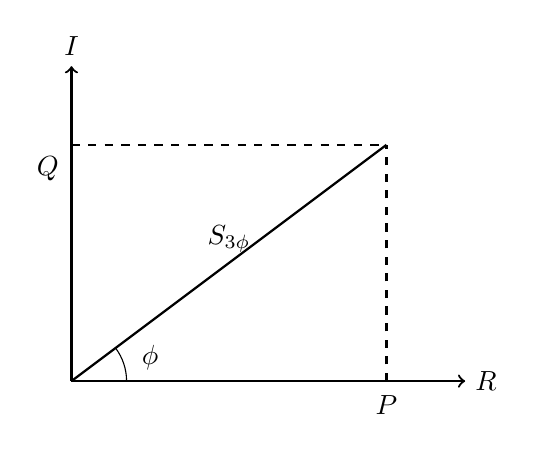
\begin{tikzpicture}

        % Ejes
        \draw[->, thick] (0,0) -- (5,0) node[right] {$\mathbb{R}$};
        \draw[->, thick] (0,0) -- (0,4) node[above] {$\mathbb{I}$};
        
        % Vectores y líneas punteadas
        \draw[thick] (0,0) -- (4,3) node[midway, above] {$S_{3\phi}$};
        \draw[dashed, thick] (4,0) -- (4,3);
        \draw[dashed, thick] (0,3) -- (4,3);
        
        % Ángulo phi
        \draw (0.7, 0) arc[start angle=0, end angle=36.87, radius=0.7];
        \node at (1, 0.3) {$\phi$};
        
        % Etiquetas de los ejes
        \node at (4, -0.3) {$P$};
        \node at (-0.3, 2.7) {$Q$};
        
        \end{tikzpicture}
    \end{center}
    Donde Q corresponde a la potencia reactiva y P a la potencia real (La que realmente utiliza la carga para operar y que buscamos maximizar).Luego podemos relacionar la potencia $S_{3\phi}$ tal que:
    \begin{align}
        cos(\phi) &= \frac{P}{S_{3\phi}}\\
        FP \cdot S_{3\phi}&= P\\
        \|S_{3\phi}\| = \left|\frac{P}{FP} \right| &= 900[kVA]
    \end{align}
    (Se utiliza que $\cos(\phi) = FP$).Por tanto que $S_{3\phi}$ se puede denotar como:
    \begin{align}
        S_{3\phi} &= 900 \angle 36.87^{\circ} [kVA]
    \end{align}
    y por lo tanto para una fase tenemos que 
    \begin{align}
        S_{1\phi} &= \frac{900}{3} \angle 36.87^{\circ} [kVA]\\
        S_{1\phi} &= 300 \angle 36.87^{\circ} [kVA]
    \end{align}
    Asi tenemos que por tanto su equivalente monofasico vendra dado por:
    \begin{center}
        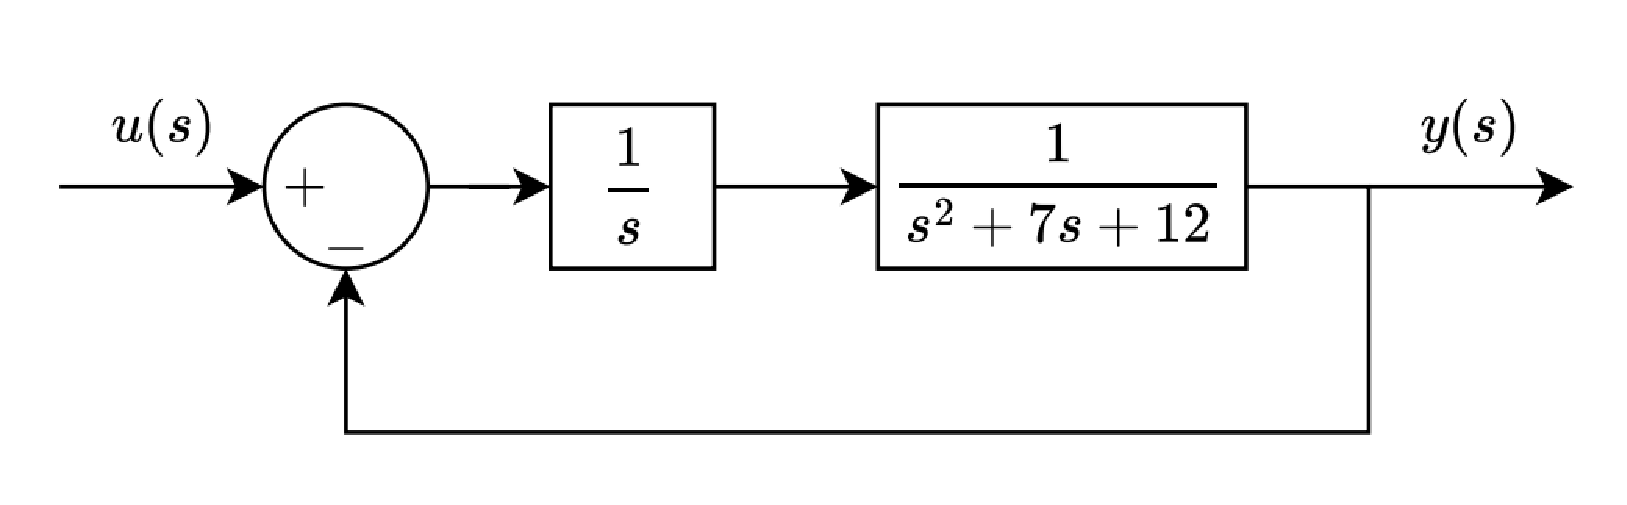
\includegraphics[width=0.55\textwidth]{Auxiliar_1_2}
        \captionof{figure}{Esquema General Monofasico}
      \end{center}
    Dado que la potencia S como el voltaje son conocidos, es posible determinar la corriente mediante mallas, tal que:
    \begin{align}
        S &= V \cdot I^{*} 
    \end{align}
    Como buscamos obtener la corriente debemos tener el cuidado con el conjugado, dado que nos afectara a la fase con un signo negativo o lo equivalente a realizar una rotacion fasorial, luego:
    \begin{align}
        I = \left( \frac{S}{V}\right)^{*} = \left(125 \angle 36.87^{\circ}\right)^{*}\,[\text{A}] = 125 \angle -36.87^{\circ}\,[\text{A}]
    \end{align}
    \begin{center}
        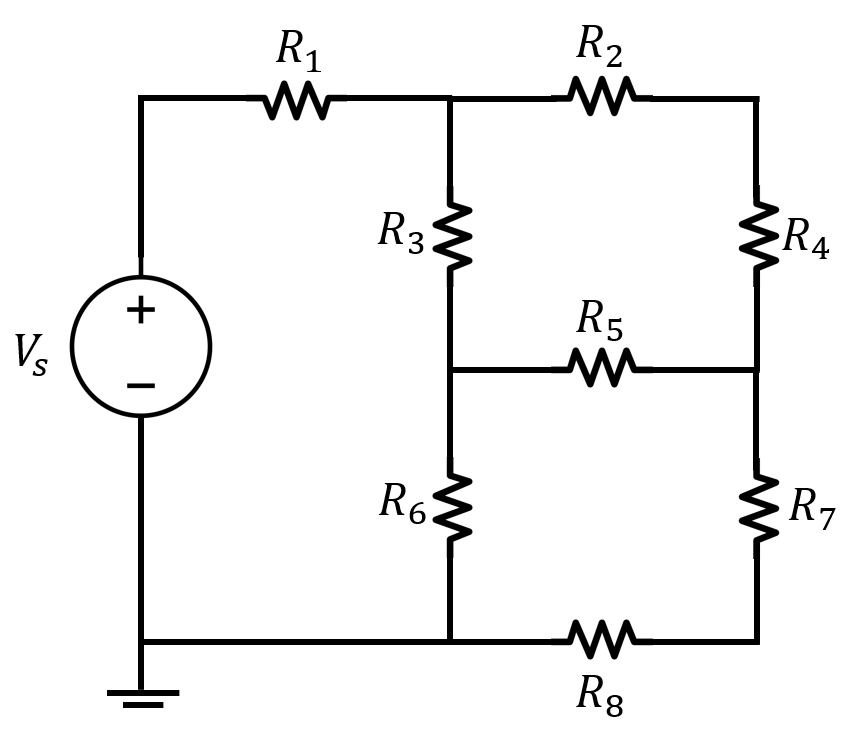
\includegraphics[width=0.55\textwidth]{Auxiliar_1_3}
        \captionof{figure}{Esquema General Monofasico}
      \end{center}
    Con lo que ahora es posible utilizar metodo de mallas para obtener el voltaje que suministra el generador ($V_{a}$) como: 
    \begin{align}
      -V_{a} &+ (0.8 + j6.4) \cdot 125 \angle -36.87^{\circ} + 2400 = 0\\
      V_{a} &= 3016.28 \angle 11.09^{\circ} [V]
    \end{align}
Finalmente se obtiene lo buscado, es importante que notemos la gran diferencia de voltaje existente entre la carga y el generador.Esto debido a la cantidad de potencia perdida en su componente reactiva esto se logra compensar mediante un banco de condensador para cancelar esta componente.
\subsection*{Resolucion 1.2}
Luego al adicionar un banco de condensador, y como analizamos la componente unicamente monofasica, tendremos que el esquema vendra dado:
\begin{center}
    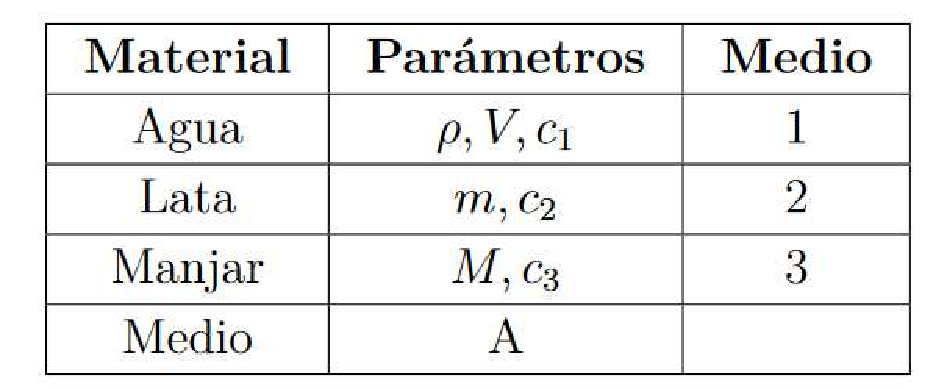
\includegraphics[width=0.6\textwidth]{Auxiliar_1_4}
    \captionof{figure}{Esquema General Monofasico con Condensador}
  \end{center}
Dado que nos dan la potencia reactiva $Q_{3\phi}$ al igual que las relaciones ya vistas, tenemos que $Q_{1\phi} = \frac{Q_{3\phi}}{3} =\frac{576}{3}= 192[KVar]$. Ademas es importante tener en cuenta que I seguira manteniendose dado que la potencia consumida por la carga sigue siendo la misma, esto aplica tanto para el voltaje como la corriente dado que ambos se relacionan para S. Luego tenemos por tanto que mediante kirchoff $i_{1}+i_{c} = I$, con lo que deberemos obtener $i_{1}$ , pero dado que tenemos la potencia reactiva $Q_{1\phi}$ y el condensador no tiene potencia P, luego:
\begin{align}
    i_{c} = \left(\frac{S}{V_{c}}\right)^{*} = \left( \frac{jQ_{1\phi}}{V_{c}}\right) = 80 \angle -90^{\circ} [A] 
\end{align}
Con lo que ahora es posible obtener $i_{1}$ como:
\begin{align}
    i_{1} + i_{c} =& I\\
    i_{1} =&  I- i_{c} = 125 \angle -36.87^{\circ} - 80\angle -90^{\circ} = 100.1248 \angle 2.86^{\circ} [A] 
\end{align}
De esta manera es posible obtener el voltaje en la carga mediante metodo de mallas, con lo que:
\begin{align}
    -V_{a} &+ i_{i}(0.8 + j6.4)+ 2400 = 0\\
    V_{a} &= 2531.317 \angle 14.74^{\circ} [V]
\end{align}
Con lo que se obtiene un voltaje mas cercano al anterior, con lo que no existe una diferencia excesiva a diferencia de antes.
\subsection*{Resolucion 1.3}
Se busca obtener la eficienciadel suministro de potencia activa en el primer caso, para esto se debe tener en cuenta que la eficiencia se define como:
\begin{align}
    \eta = \frac{P_{carga}}{P_{generador}} =  \frac{P_{\text{Potencia que se consume}}}{P_{\text{Potencia que se genera}}}
\end{align}
Para el primer caso se tendra que en base al esquema:
\begin{center}
    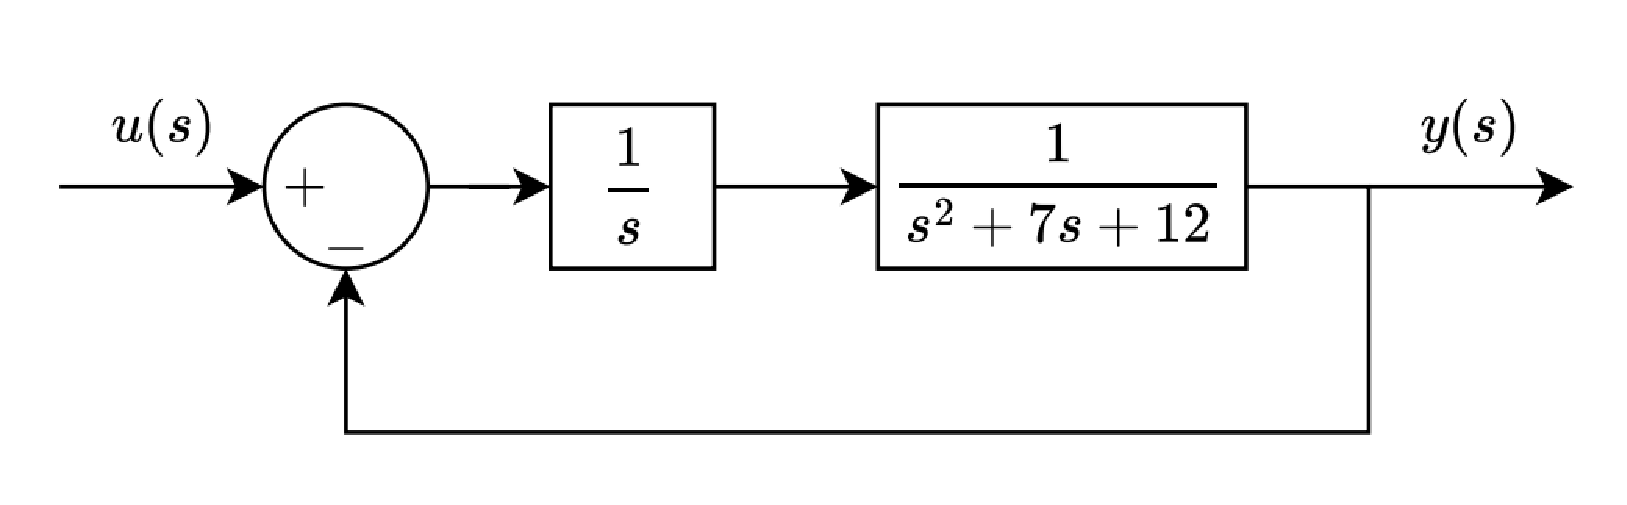
\includegraphics[width=0.5\textwidth]{Auxiliar_1_2}
    \captionof{figure}{Esquema General Monofasico}
  \end{center}
Por enunciado se tendra que la potencia trifasica consumida es de 720[Kw], con lo que en monofasico tendermos que $P_{1\phi} = \frac{720}{3} = 240[kW] $ , con lo que se tiene que la eficiencia es:
\begin{align}
    \eta = \frac{240}{240 + P_{\text{Perdidas}}}
\end{align}
Donde la potencia de las perdidas se puede obtener de manera directa mediante
\begin{align}
    P_{\text{Perdidas}} = |I|^{2}R = |125 \angle -36.87^{\circ}|^{2} \cdot 0.8 = 12.5[KW]
\end{align}
Con lo que se obtiene que la eficiencia es de:
\begin{align}
    \eta = \frac{240}{240 + 12.5} = 0.95
\end{align}
Con lo que la eficiencia en terminos de porcentaje corresponde a un 95\%.
\subsection*{Resolucion 1.4}
Para el analizar el segundo caso, procdeimiento es analogo con lo que se obtiene que:
\begin{align}
    P_{\text{Perdidas}} = |I|^{2}R = |100.1248 \angle 2.86^{\circ}|^{2} \cdot 0.8 = 8.01[KW]
\end{align}
Con lo que la eficiencia vendra dada por:
\begin{align}
    \eta = \frac{240}{240 + 8.01} = 0.967
\end{align}
Con lo que la eficiencia en terminos de porcentaje corresponde a un 96.7\%, donde se logra observar una mejoria con respecto al caso anterior, si bien no es una mejoria significativa, se logra disminuir las perdidas en el sistema.
\subsection*{Resolucion 1.5}
Finalmente para obtener el tamaño de los condensadores, se debe tener en cuenta que la potencia reactiva se puede relacionar con la corriente y el voltaje mediante:
\begin{align}
    S = V \cdot I^{*} = \frac{|V|^{2}}{Z^{*}}
\end{align}
Que para el caso de un condensador tenemos que:
\begin{align}
    -jQ_{c} &= \frac{|V|^{2}}{jx_{c}} \\
    x_{c} &= \frac{|V|^{2}}{Q_{c}} \\
    x_{c} &= \frac{2400^{2}}{192} \\
    x_{c} &= 30\,[\Omega]
\end{align}
Con lo que finalmente tenemos:
\begin{align}
    x_{c} &= \frac{1}{wC} \\
    C &= \frac{1}{wX_{c}}\\
    C &= \frac{1}{2\pi \cdot 60 \cdot 30} = 88.4[\mu F] 
\end{align}
De esta manera se obtiene el tamaño de los condensadores.
    \end{solution}
    %%%%%%%%%%%%%%%%%%%%%%%%%%%
    \question Se tiene el siguiente sistema trifasico equilibrado en secuencia positiva
    \begin{enumerate}
        \item Determine la forma y los parametros del circuito equivalente monofasico.
        \item Determinar las corrientes que circulan por las cargas y las corrientes de linea.
        \item Calcular la potencia aparente, activa y reactiva de cada carga, y su respectivo factor de potencia.
    \end{enumerate}
    Considere los siguientes datos:
    \begin{align}
        V_{ff} &= 400[V] \\
        Z_{1} &= 150 + j90[\Omega] \\
        Z_{2} &= 82.4621\angle 14.03^{\circ}[\Omega]
    \end{align}
    \begin{figure}[h!]
        \centering
        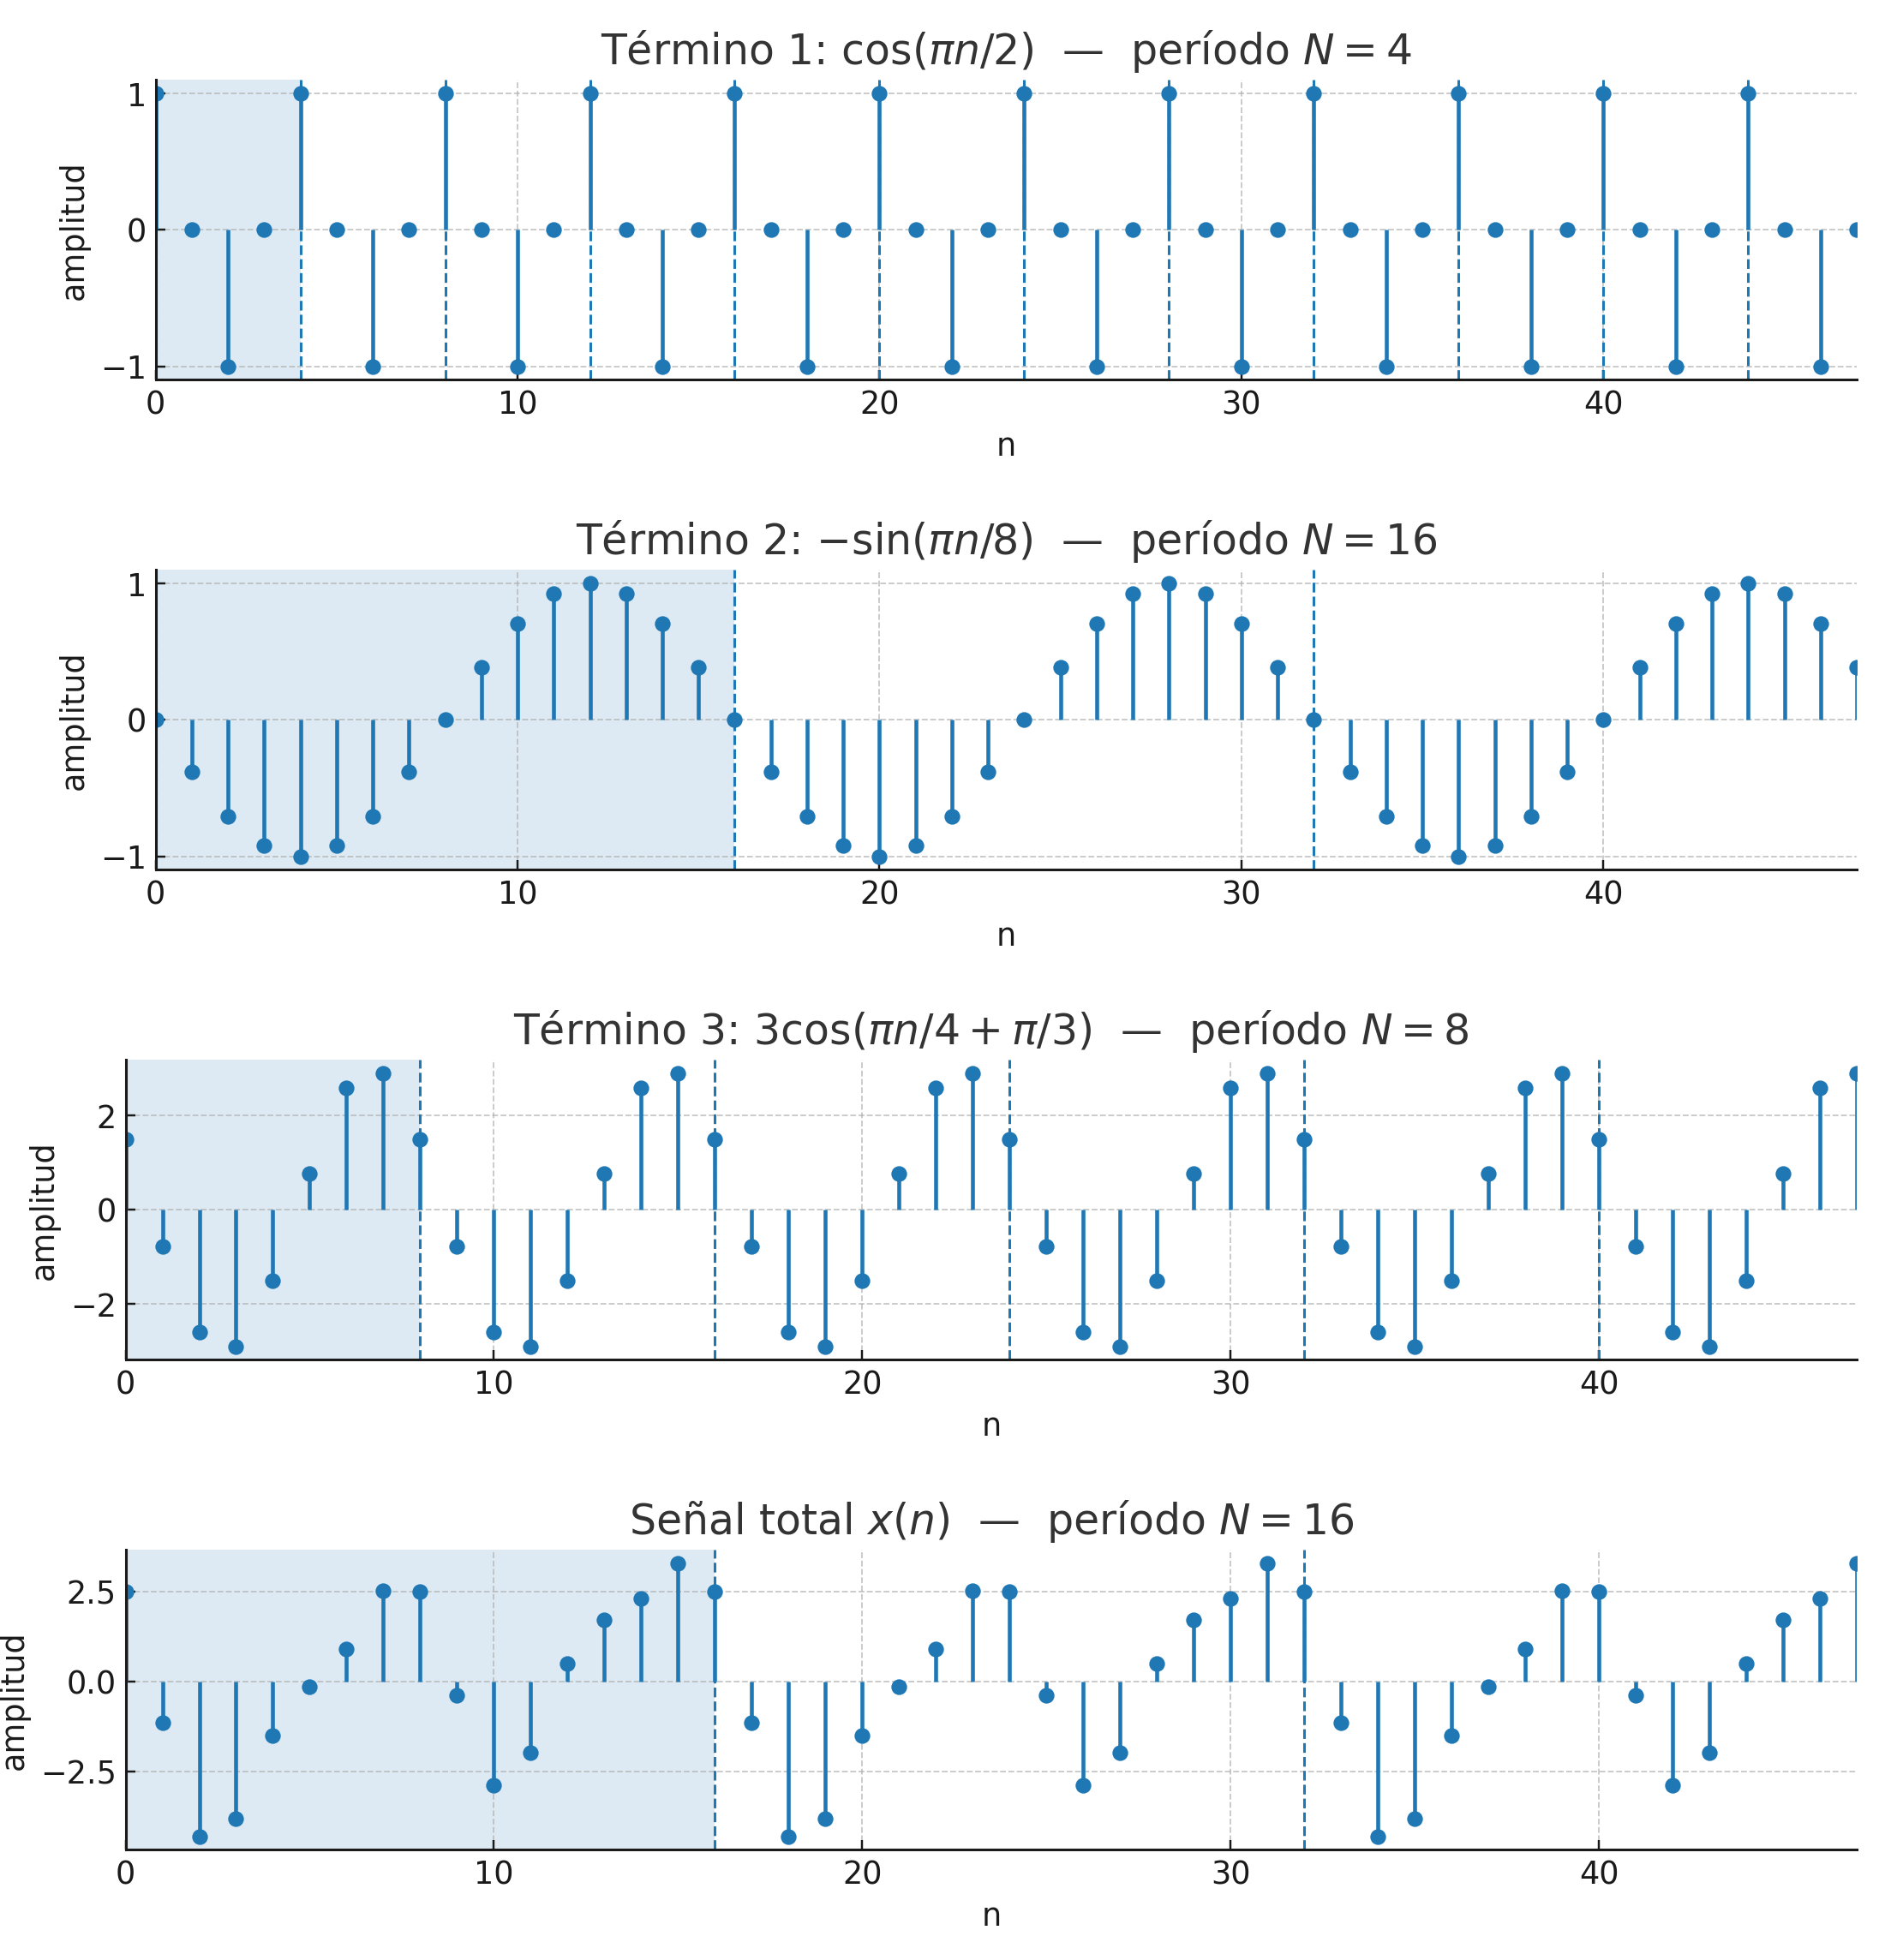
\includegraphics[width=0.5\textwidth]{Auxiliar_1_1}
    \end{figure}
%%%%%%%%%%%%%%%%%%%%%%%%%%%
\begin{solution}
\subsection*{Resolucion 2.1}
    Similar al ejercicio anterior, es necesario el pasar el sistema a su equivalente monofasico,por lo que deberemos pasar todo a a una configuracion en estrella.
    \begin{align}
        V_{fn} &= \frac{V_{ff}}{\sqrt{3}}\angle -30^{\circ} 
               = \frac{400}{\sqrt{3}} \angle -30^{\circ} 
               = 230.9401 \angle -30^{\circ}[V]
    \end{align}
Una vez obtenidos los voltajes Fase-Neutro, deberemos realizar lo analogo para obtener las impedancias en estrella, con lo que se obtiene lo siguiente:
\begin{align}
    Z^{'}_{1}= \frac{Z_{1}}{3} = \frac{150 + j90}{3}= 50 + j30 = 58.31 \angle 30.96^{\circ} [\Omega]
\end{align}
De esta manera el circuito adopta la siguiente forma:
\begin{center}
    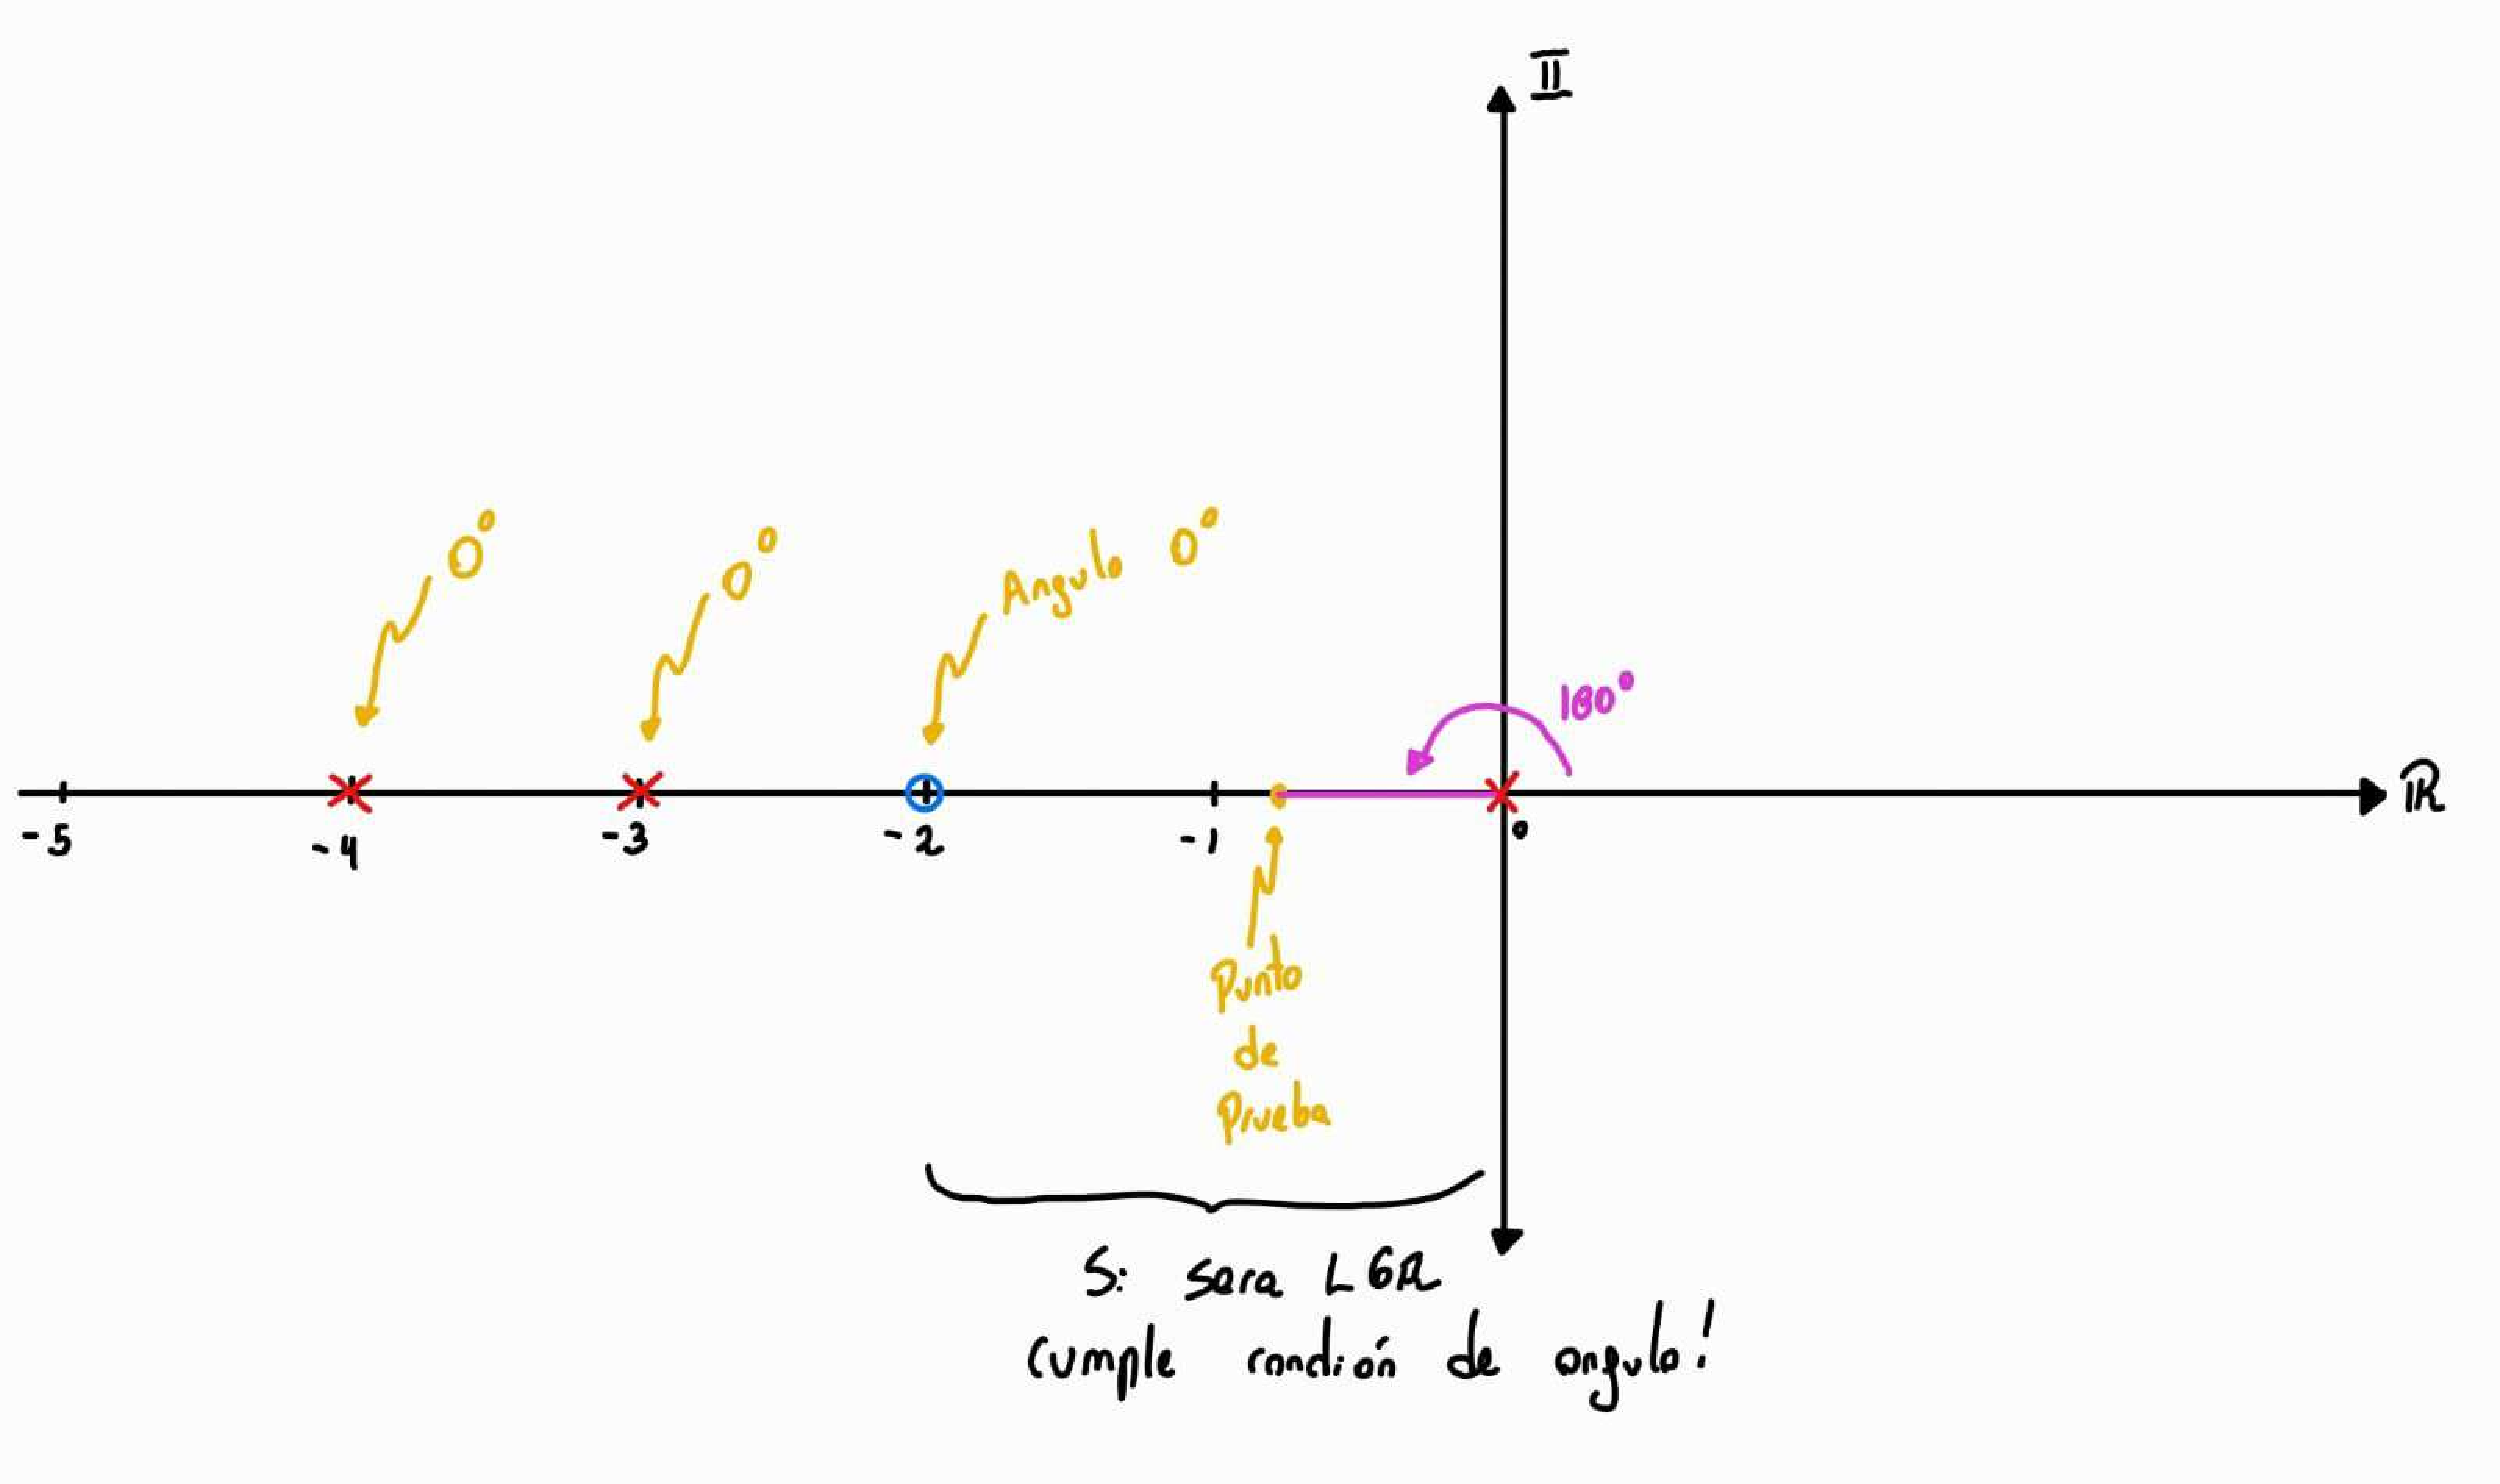
\includegraphics[width=0.6\textwidth]{Auxiliar_1_5}
    \captionof{figure}{Esquema General Monofasico}
  \end{center}
Con lo que el circuito permite reordenarse de manera simple como un circuito con dos impedancias en paralelo y una fuente de voltaje $V_{fn}$ tal que:
\begin{center}
    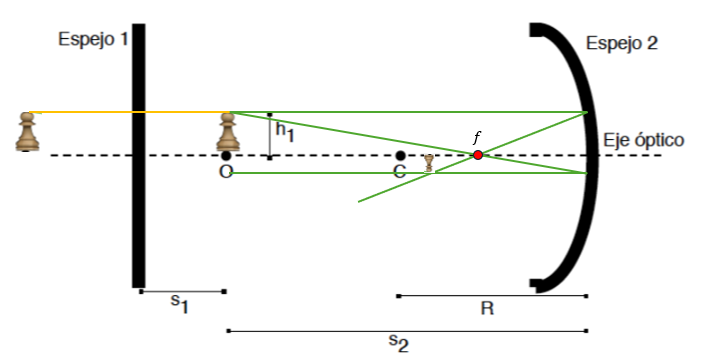
\includegraphics[width=0.5\textwidth]{Auxiliar_1_6}
    \captionof{figure}{Esquema General Monofasico}
  \end{center}
\subsection*{Resolucion 2.2}
Se busca obtener las diferentes corriente que circulan tanto por la carga y por las corrientes de linea, por lo que, de manera directa se tendra lo siguiente:
\begin{align}
    I_{1} &= \frac{V_{fn}}{Z^{'}_{1}}\\
          &= \frac{230.9401 \angle -30^{\circ}}{58.31 \angle 30.96^{\circ}}\\
            &= 3.96 \angle -61.96^{\circ} [A]
\end{align}
Por otro lado, para la corriente que circula por la segunda impedancia se tiene que:
\begin{align}
    I_{2} &= \frac{V_{fn}}{Z_{2}}\\
          &= \frac{230.9401 \angle -30^{\circ}}{82.4621 \angle 14.03^{\circ}}\\
            &= 2.8 \angle -44.03^{\circ} [A]
\end{align}
Finalmente para obtener la corriente de linea se tiene que:
\begin{align}
    I_{linea} &= I_{1} + I_{2}\\
              &= 3.96 \angle -61.96^{\circ} + 2.8 \angle -44.03^{\circ}\\
              &= 3.94\angle 54^{\circ} [A]
\end{align}
De esta manera se obtiene finalmente las corrientes de linea y de cada impedancia.
\subsection*{Resolucion 2.3}
Finalmente se busca obtener la potencia aparente, activa y reactiva de cada carga, y su respectivo factor de potencia, para esto se tiene que considerar lo visto anterioremente como:
\subsubsection*{Primera carga}
\begin{align}
    S_{1\phi} &= V_{fn} \cdot I^{*}\\
    &= 230.9401 \angle -30^{\circ} \cdot 3.96 \angle 61.96^{\circ}\\
    &= 914.453 \angle 30.96^{\circ} [VA]\\
    &= 784.33 + j470.32 [VA]
\end{align}
Donde similar al ejercicio anterior, se tendra una potencia real P asociada a los 784.33 [W] y una potencia reactiva Q asociada a los 470.32 [VAr], con lo que se tiene que el factor de potencia es:
\begin{align}
    FP = \cos(\phi) = \frac{P}{S} = \frac{784.33}{914.453} = 0.857
\end{align}
Notamos que es inductivo dado que el angulo de la potencia es positivo, por otro lado para la segunda carga se tiene un procedimiento analogo:
\subsubsection*{Segunda carga}
\begin{align}
    S_{1\phi} &= V_{fn} \cdot I^{*}\\
    &= 230.9401 \angle -30^{\circ} \cdot 2.8 \angle 44.03^{\circ}\\
    &= 627.65 \angle 14.03^{\circ} [VA]\\
    &= 627.5 + j 156.5 [VA]
\end{align}
Con lo que se tiene que el factor de potencia es:
\begin{align}
    FP = \cos(\phi) = \frac{P}{|S|} = \frac{627.5}{646.65} = 0.9701
\end{align}
Al igual que antes observamos que es inductivo dado que el angulo de la potencia es positivo, con lo que se obtiene la potencia aparente, activa y reactiva de cada carga, y su respectivo factor de potencia.
\end{solution}
%%%%%%%%%%%%%%%%%%%%%%%%%%%
\question La potencia trifásica total suministrada a una carga trifásica equilibrada cuando está operando a una tensión de fase-fase de \(220 \, [\text{kV}]\) es de \(800 \, [\text{kW}]\) con un factor de potencia de \(0,8\) en retardo. La impedancia de la línea de distribución que alimenta a la carga es de \(80 + j640 \, [\Omega/\text{fase}]\) y la frecuencia de la red es de \(50 \, [\text{Hz}]\).Considerando lo anterior, responda las siguientes preguntas:
\begin{enumerate}
    \item[(a)] ¿Cuál es la magnitud de la tensión en el extremo de la línea correspondiente al generador cuando la carga está operando con una tensión fase-fase de \(220 \, [\text{kV}]\)?
    \item[(b)] ¿Cuál debería ser la capacidad nominal en kVAr de 3 condensadores conectados en Estrella en paralelo con la carga para que eleven el factor de potencia a atrasado de 0.95?
    \item[(c)] ¿Cuál debe ser la capacitancia de cada condensador del inciso (b)?
\end{enumerate}
%%%%%%%%%%%%%%%%%%%%%%%%%%%
\begin{solution}
    \subsection*{Resolucion 3.1}
    Se busca obtener la magnitud de la tensión en el extremo de la línea correspondiente al generador, esto al igual que lo visto con anterioridad, por lo que se tiene el siguiente esquema:
    \begin{center}
        \begin{circuitikz}

            % Rectángulo izquierdo
            \draw (0, 0) rectangle (2, 4) node[midway] {$S_{3\phi}$};
            
            % Rectángulo derecho
            \draw (6, 0) rectangle (9, 4);
            
            % Etiquetas dentro del rectángulo derecho
            \node at (7.5, 2.8) {FP = 0.8};
            \node at (7.5, 2.2) {$P = 800 \, [kW]$};
            
            % Impedancias
            \draw (2,3.5) to[generic, l=$Z$] (6,3.5);
            \draw (2,2) to[generic, l=$Z$] (6,2);
            \draw (2,0.5) to[generic, l=$Z$] (6,0.5);
            
            % Flecha y voltaje en el rectángulo de arriba
            \draw[->] (5,3.5) -- (5,2.5) node[right] {$V_{line}$};
            
            \end{circuitikz}
        \end{center}
Luego se busca obtener $S_{1\phi}$, para poder asociarlo a la corriente del sistema monofasico, por lo que:
\begin{align}
    \cos(\phi) = FP = \frac{P}{S_{3\phi}}
\end{align}
Con lo que tenemos
\begin{align}
    |S_{3\phi}| = \frac{P}{FP} = \frac{800}{0.8} = 1000[kVA]
\end{align}
Luego para el angulo se obtiene directamente:
\begin{align}
    \phi = \arccos(0.8) = 36.87^{\circ}
\end{align}
De esta manera tenemos que $S_{1\phi}$:
\begin{align}
    S_{1\phi} = \frac{1000}{3} \angle 36.87^{\circ} = 333.33 \angle 36.87^{\circ} [kVA]
\end{align}
Luego se tiene que pasar al sistema monofasico, con lo que la impedancia vendra dada por:
\begin{align}
    V_{fn} = \frac{220}{\sqrt{3}}[\Omega]
\end{align}
Con lo que el esquema vendra dado por:
\begin{center}
    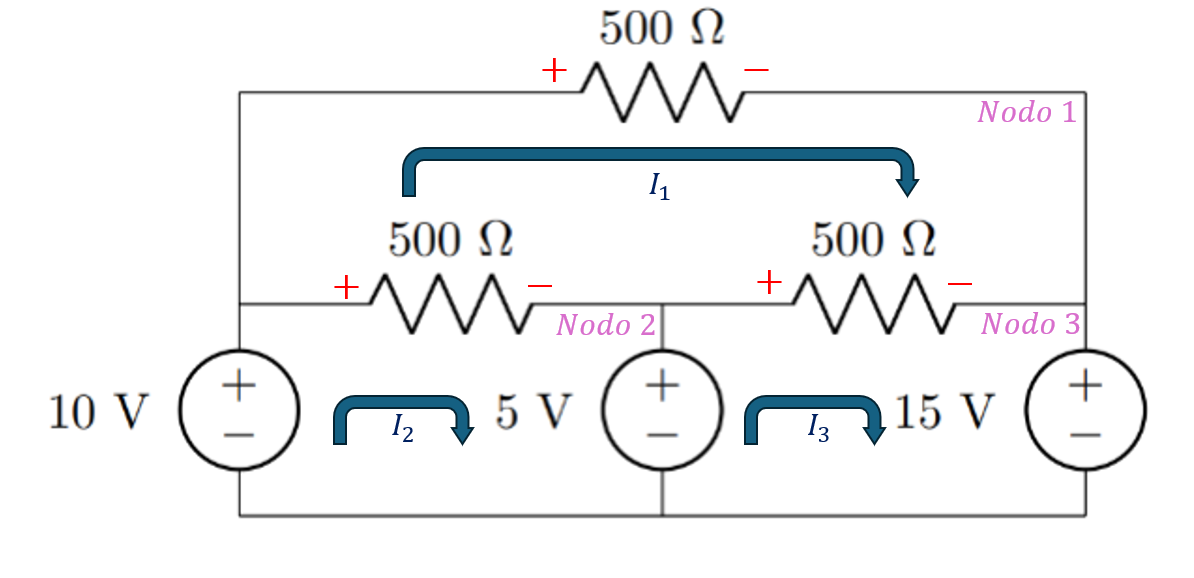
\includegraphics[width=0.5\textwidth]{Auxiliar_1_7}
    \captionof{figure}{Esquema General Monofasico}
  \end{center}
Luego el voltaje la corriente se obtiene como:
\begin{align}
    S_{1\phi} &= V_{fn} \cdot I^{*}\\
    I &= \left(\frac{S_{1\phi}}{V_{fn}}\right)^{*}\\
    &= 2.64 \angle -36.87^{\circ} [A]
\end{align}
Con lo que finalmente el voltaje del generador se tendar que mediante malla:
\begin{align}
    -V_{a} &+ (80 + j640) \cdot 2.64 \angle -36.87^{\circ} + \frac{220}{\sqrt{3}} = 0\\
    V_{a} &= 128.199\angle 0.5^{\circ} [V]
\end{align}
Con lo que se obtiene el voltaje del generador.
\subsection*{Resolucion 3.2}
Se busca aumentar el factor de potencia a 0.95, con lo que podemos formular un esquema tal que:
\begin{center}
    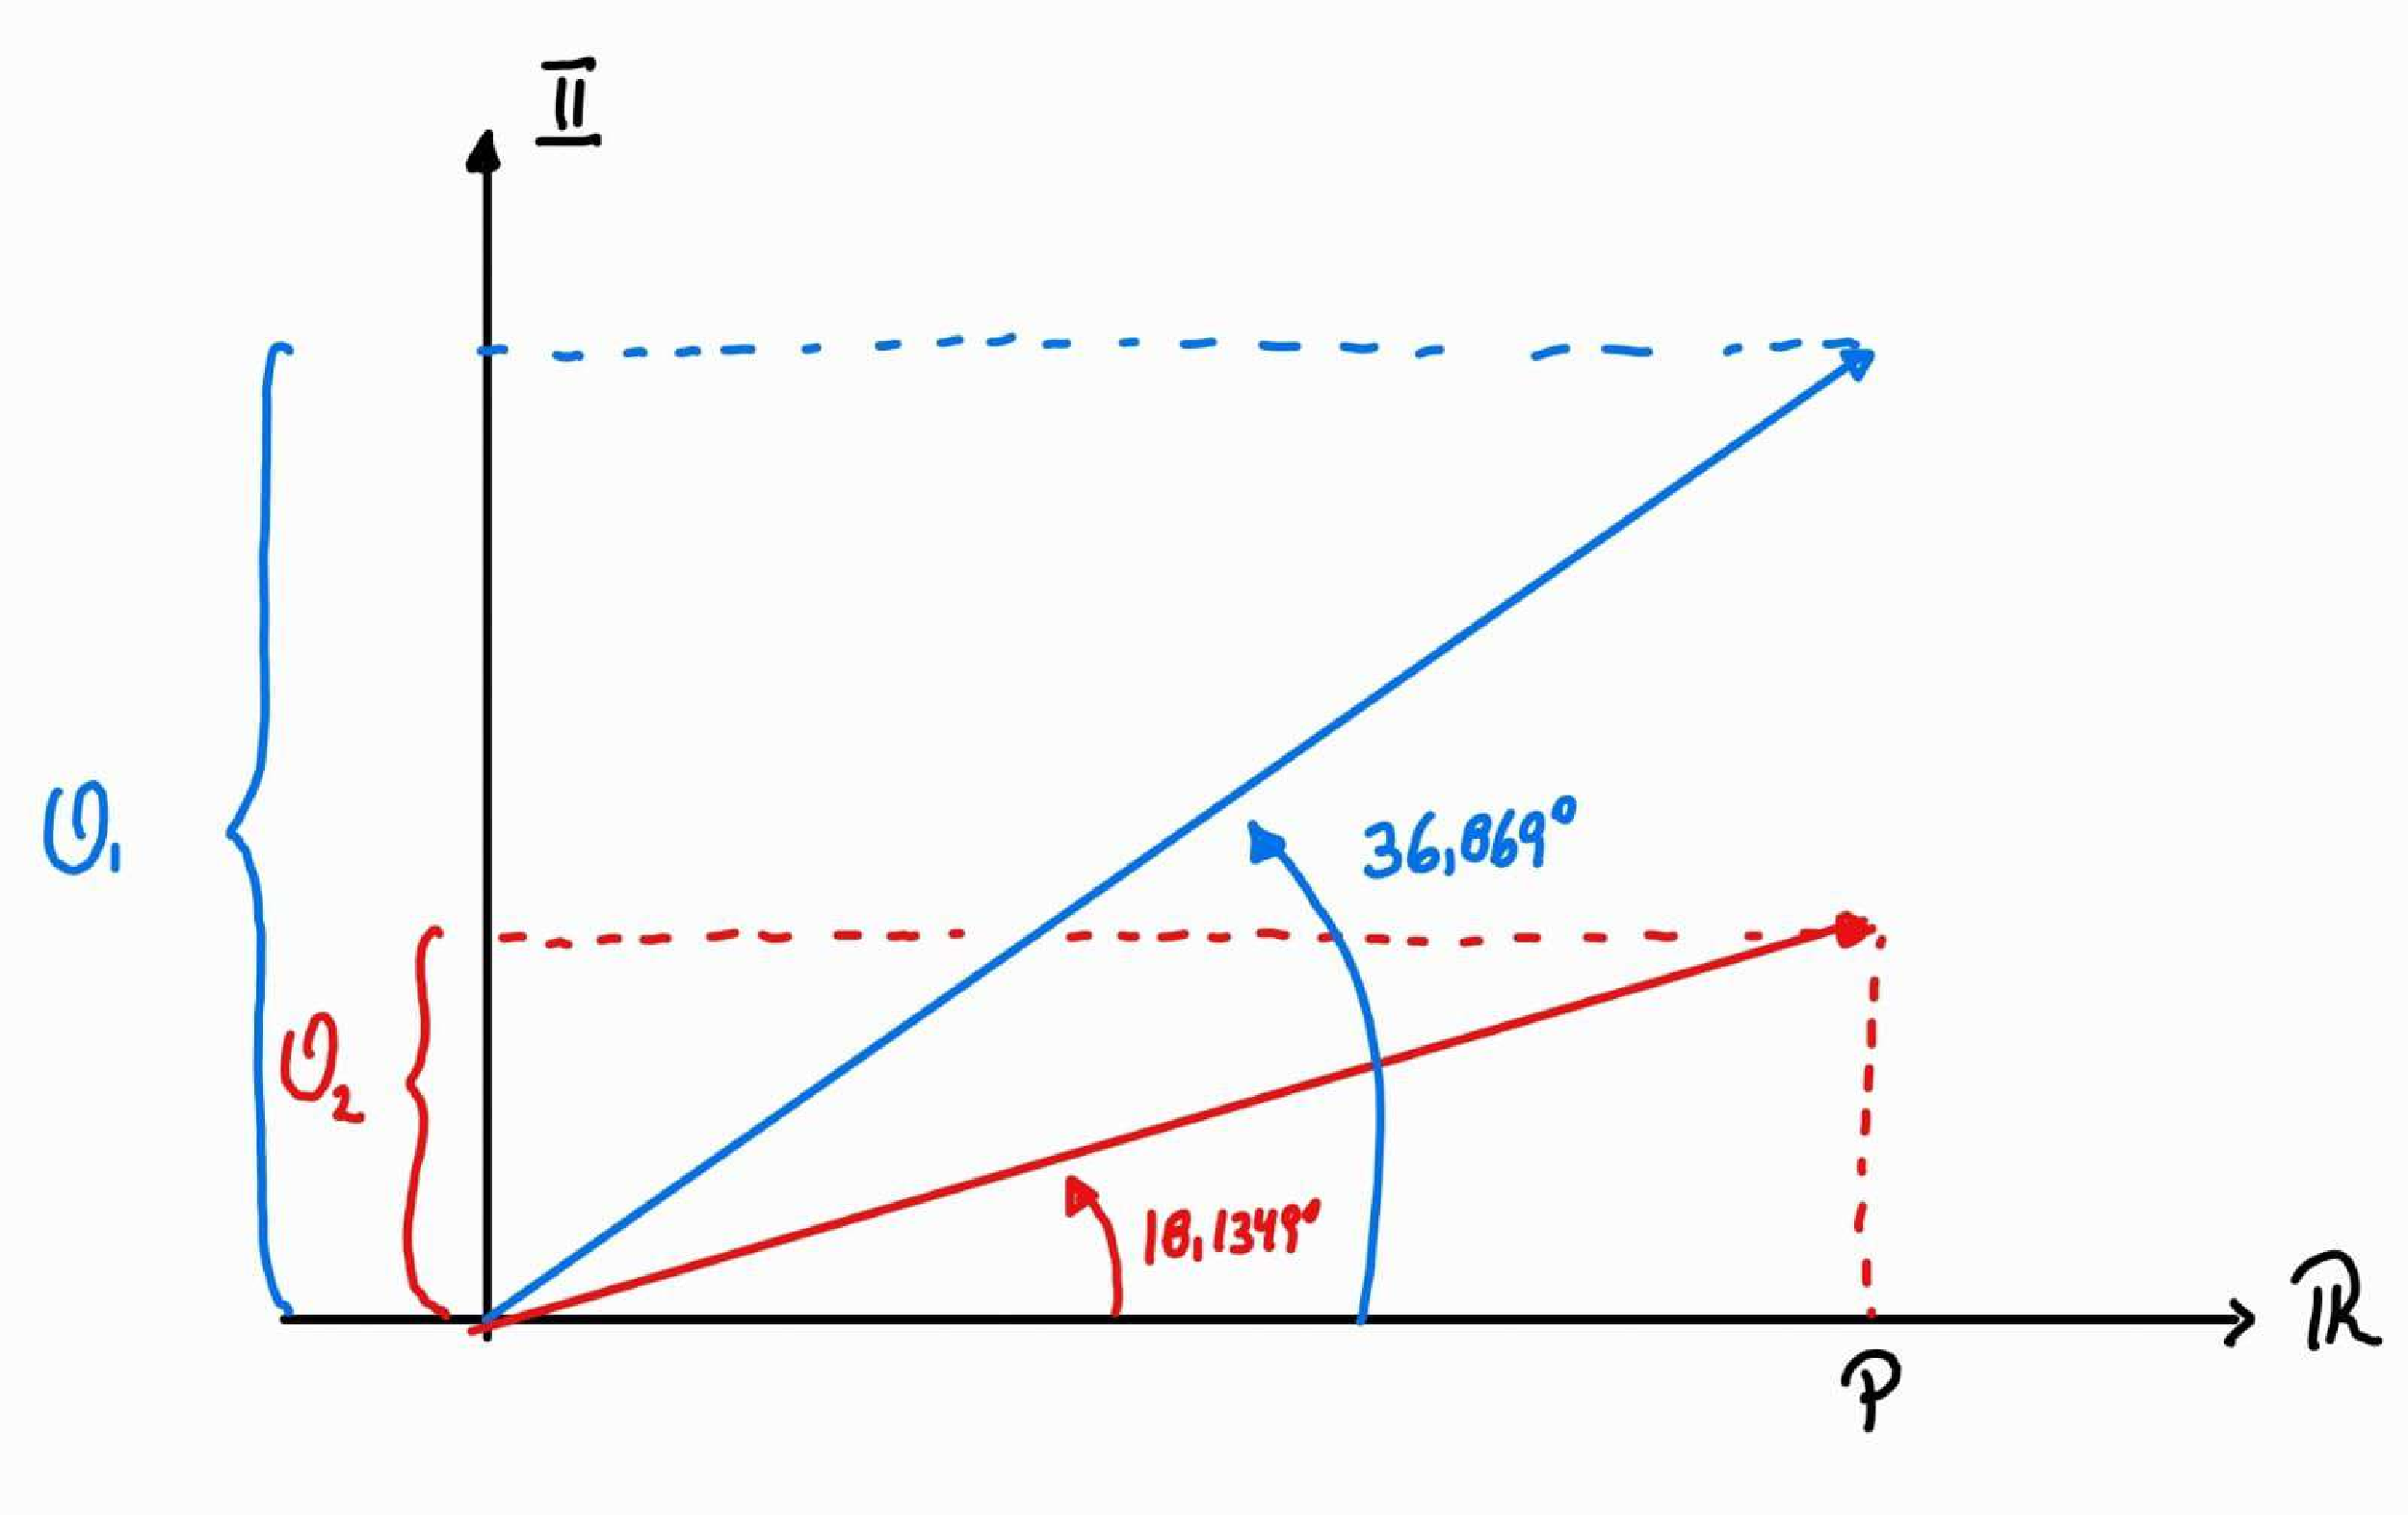
\includegraphics[width=0.4\textwidth]{Auxiliar_1_8}
    \captionof{figure}{Esquema potencias reactivas}
  \end{center}
Luego el factor de potencia en rojo vendra dado por:
\begin{align}
    FP&= 0.95\\
    \phi &= \arccos(0.95) = 18.19^{\circ}
\end{align}
Mientras que el factor de potencia asociado a el azul vendra dado por:
\begin{align}
    FP &= 0.8 \\
    \phi &= \arccos(0.8) = 36.87^\circ
\end{align}
Luego se tendremos que reducir la potencia reactiva de la carga tal que:
\begin{align}
    Q_{3\phi} &= Q_{1} - Q_{2} = 600 - 263.03 = 336.97 [KVar]\\
    Q_{1\phi} &= \frac{Q_{3\phi}}{3} = 112.32 [KVar]
\end{align}
Con lo que se obtiene que la potencia reactiva de cada condensador es de 112.32 [KVar].
\subsection*{Resolucion 3.3}
Se busca obtener la capacitancia de cada condensador al igual que antes tenemos que:
\begin{align}
    -jQ_{c} &= \frac{|V|^{2}}{jX_{c}}
\end{align}
Con lo que tenemos que 
\begin{align}
    Q_{c} &= V_{fn}^{2}wC\\
\end{align}
Luego despejando la capacitancia C considerando una frecuencia de 50[Hz] se obtiene un valor de C=22.2[n F]
\end{solution}
%%%%%%%%%%%%%%%%%%%%%%%%%%%

\end{questions}
\newpage
%%%%%%%%%%%%%%%%%%%%%%%%%%%
\section{Resumen}

\section*{Fasores}

Considerando una onda sinusoidal del tipo:
\begin{align}
v(t) &= V_m \cos(\omega t + \phi)
\end{align}
Donde:
\begin{itemize}
    \item $V_m$ es la magnitud de la onda.
    \item $\omega$ es la frecuencia en [rad/seg].
    \item $\phi$ es la fase de la onda en [rad].
\end{itemize}
Se tendrá que la representación fasorial de la onda anterior será:
\begin{align}
\tilde{V} &= V e^{j\phi} = V \angle \phi
\end{align}
Donde $V$ corresponderá a la amplitud efectiva de la onda. Por otro lado, se debe recordar que un número complejo se puede escribir como un número polar de la siguiente forma:
\begin{align}
z &= x + jy = (r \angle \phi) = r e^{j\phi}
\end{align}
Donde:
\begin{align}
r &= \sqrt{x^2 + y^2}
\end{align}
\begin{align}
\phi &= \arctan\left(\frac{y}{x}\right)
\end{align}
\begin{itemize}
    \item \textbf{Tensiones:}
    \begin{align}
        V_{\Delta} &= \sqrt{3} V_Y \angle 30^\circ \\
        V_f &= \frac{V_{\Delta}}{\sqrt{3}} \angle -30^\circ
    \end{align}
    Por ejemplo:
    \begin{align}
        \Rightarrow V_{ab} &= \sqrt{3} V_{an} \angle 30^\circ
    \end{align}
    
    \item \textbf{Corrientes:}
    \begin{align}
        I_Y &= \sqrt{3} I_{\Delta} \angle 30^\circ \\
        I_{\Delta} &= \frac{I_Y}{\sqrt{3}} \angle -30^\circ
    \end{align}
    Por ejemplo:
    \begin{align}
        \Rightarrow I_{an} &= \sqrt{3} I_{ab} \angle 30^\circ
    \end{align}
    
    \item \textbf{Impedancias:} \\
    Asumiendo que el sistema es equilibrado, es decir, que las cargas son iguales, se tendrá:
    \begin{align}
        Z_Y &= \frac{Z_{\Delta}}{3}
    \end{align}
\end{itemize}

\begin{itemize}
    \item \textbf{Impedancias:} \\
    Asumiendo que el sistema es equilibrado, es decir, que las cargas son iguales, se tendrá:
    \begin{align}
        Z_Y &= \frac{Z_{\Delta}}{3}
    \end{align}
\end{itemize}

\section*{Potencias trifásicas}

\begin{itemize}
    \item \textbf{Aparente:}
    \begin{align}
        S_{1\phi} &= V_{fn} \cdot I_{f} = P_{1\phi} + jQ_{1\phi} \\
        S_{3\phi} &= 3 \cdot S_{1\phi}
    \end{align}
    
    Donde:
    \begin{itemize}
        \item $S_{1\phi}$ es la potencia aparente monofásica medida en Volt-Ampere [VA].
        \item $P_{1\phi}$ es la potencia activa monofásica medida en Watts [W].
        \item $Q_{1\phi}$ es la potencia reactiva monofásica medida en Volt-Ampere reactivos [VAr].
    \end{itemize}
    
    \item \textbf{Activa y reactiva:}
    \begin{align}
        P_{1\phi} &= \text{Re}\{V_{fn} \cdot I_{f}^*\} = |S_{1\phi}|\cos(\phi) \\
        Q_{1\phi} &= \text{Im}\{V_{fn} \cdot I_{f}^*\} = |S_{1\phi}|\sin(\phi)
    \end{align}
    
    Donde $\phi = \text{arccos}(FP)$ corresponde al desfase angular, y $FP$ corresponderá al factor de potencia.
    
\end{itemize}

\section*{Factor de potencia}

Se define el factor de potencia como razón entre la potencia activa y el módulo de la potencia aparente.

\begin{align}
FP &= \cos(\phi) = \frac{P}{|S|}
\end{align}

Cabe destacar que el factor de potencia va siempre acompañado de un “apellido”, el cual indica si el fasor de la corriente está atrasado o adelantado con respecto al fasor del voltaje, lo que afecta al signo del ángulo $\phi$.

\begin{itemize}
    \item Un factor de potencia en \textbf{adelanto} significa que el fasor de la corriente se adelanta con respecto al fasor del voltaje, lo cual indica que estamos en presencia de una \textbf{impedancia capacitiva} y que el signo del ángulo $\phi$ va a ser negativo.
    \item Un factor de potencia en \textbf{atraso} significa que el fasor de la corriente se atrasa con respecto al fasor del voltaje, lo cual indica que estamos en presencia de una \textbf{impedancia inductiva} y que el signo del ángulo $\phi$ es positivo.
\end{itemize}
\end{document}